\documentclass{article}
\usepackage{amsmath}
\usepackage{graphicx}
\usepackage{subcaption}
\usepackage{setspace}
\usepackage[backend=bibtex,style=verbose-trad2]{biblatex}
\usepackage{siunitx}
\usepackage{multirow}
\usepackage{booktabs}
\usepackage{longtable}
\usepackage{rotating}
\usepackage{pgfplotstable}
\usepackage{listings}
\usepackage{color}
\usepackage{hyperref}
\usepackage{enumitem}

\begin{document}
\newpage
\pagenumbering{arabic}

\section{Analysis}
\subsection{Background}
Mr Myslov is a teacher at Tonbridge School, and currently runs the school chess club. Seldomly, a field day event will be held, in which the club convenes together, playing a chess, or another variant, tournament. This year, Mr Myslov has decided to instead, hold a tournament around another board game, namely laser chess, providing a deviation yet retaining the same familiarity of chess. However, multiple physical sets of laser chess have to be purchased for the entire club to play simultaneously, which is difficult due to it no longer being manufactured. Thus, I have proposed a solution by creating a digital version of the game.

\subsubsection{Game Description}
Laser Chess is an abstract strategy game played between two opponents. The game differs from regular chess, involving a 10x8 playing board arranged in a predefined condition. The aim of the game is to position your pieces such that your laser beam strikes the opponents Pharoah (the equivalent of a king). Pieces include:

\begin{enumerate}
\item Pharoah
    \begin{itemize}[label=(-)]
    Equivalent to the king in chess
    \end{itemize}
\item Scarab
    \begin{itemize}[label=(-)]
    2 for each colour
    Contains dual-sided mirrors, capable of reflecting a laser from any direction
    Can move into an occupied adjacent square, by swapping positions with the piece on it (even with an opponent’s piece)
    \end{itemize}
\item Pyramid
    \begin{itemize}[label=(-)]
    7 for each colour
    Contains a diagonal mirror used to direct the laser
    The other 3 out of 4 sides are vulnerable from being hit
    \end{itemize}
\item Anubis
    \begin{itemize}[label=(-)]
    2 for each colour
    Large pillar with one mirrored side, vulnerable from the other sides
    \end{itemize}
\item Sphinx
    \begin{itemize}[label=(-)]
    1 for each colour
    Piece from which the laser is shot from
    Cannot be moved
    \end{itemize}
\end{enumerate}

On each turn, a player may move a piece one square in any direction (similar to the king in regular chess), or rotate a piece clockwise or anticlockwise by 90 degrees. After their move, the laser will automatically be fired. It should be noted that a player’s own pieces can also be hit by their own laser. As in chess, a three-fold repetition results in a draw. Players may also choose to forfeit or offer a draw.

\subsection{Client Interview}

\subsection{Current solutions}
Current free implementations of laser chess that are playable online are limited, seemingly only available on \url{https://laser-chess.com/}.

\begin{figure}
    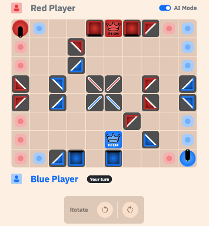
\includegraphics[width=\linewidth]{assets/laserchesscom.png}
    \caption{Online implementation on laser-chess.com}
    \label{fig:laserchesscom}
\end{figure}

The game is hosted online and is responsive and visually appealing, with pieces easy to differentiate and displaying their functionality clearly. It also contains a two-player mode for playing between friends, or an option to play against a functional CPU bot. However, the game lacks the following basic functionalities that makes it unsuitable for my client’s requests:

\begin{itemize}
\item No replay options (going through pass moves)
    \begin{itemize}
    \item A feature to look through previous moves is standard in any online chess implementation
    \item My client requires this feature as it is an essential tool in learning from past games and to aid in analyzing the course of a game and opponent’s thought process
    \end{itemize}
\item No option to save and load previous games
    \begin{itemize}
    This QOL feature allows games to be continued on if they cannot be finished in one sitting
    \end{itemize}
\item Internet connection required
    \begin{itemize}
    My client has specifically requested an offline version as the game will predominantly played in settings where a connection might not be available (i.e. on a plane)
    \end{itemize}
\item Unable to change board configuration
    \begin{itemize}
    The version of laser chess named Khet contains different starting board configurations, each offering a different style of play
    Our design will aim to append the missing feature from this website while learning from their valid UI design.
    \end{itemize}
\end{itemize}

\subsection{Objectives}
The following objectives should be met to satisfy my clients’ requirements:

\begin{enumerate}
\item All laser chess game logic should be properly implemented
    \begin{itemize}
    \item All pieces should be display correct behaviour (e.g. reflecting the laser in the correct direction)
    \item Option to rotate laser chess pieces should be implemented
    \item Pieces should be automatically detected and eliminated when hit by the laser
    \item Game should allocate alternating player’s turns
    \item Players should be able to move to an available square when it is their turn
    \item Game should automatically detect when a player has lost or won
    \item Three-fold repetition should be automatically detected
    \item Travel path of laser should be correctly implemented
    \end{itemize}
\item Save or load game options should be implemented
    \begin{itemize}
    \item Games will be encoded into FEN string format
    \item Games can be saved locally into the program files
    \item Players can load positions of previous games and continue playing
    \end{itemize}
\item Essential laser chess features should be implemented
    \begin{itemize}
    \item Essential laser chess features should be implemented
    \item Players should be able to scroll through previous moves
    \item Timer displaying time left for each player should be displayed
    \item Time logic should be implemented, pausing when it is the opponent’s turn, forfeiting players who run out of time
    \item Forfeiting should be implemented as an available option
    \end{itemize}
\item Game settings should be customizable
    \begin{itemize}
    \item Piece and board colour should be customizable
    \item Option to play CPU or another player should be implemented
    \item Starting player turn and board layout should be customizable
    \end{itemize}
\item CPU player
    \begin{itemize}
    \item CPU player should be functional and display an adequate level of play
    \item CPU should be within an adequate timeframe (5 seconds)
    \item CPU should be functional regardless of starting board position
    \end{itemize}
\item Game UI should improve player experience
    \begin{itemize}
    \item Selected pieces should be clearly marked with a surrounding circle
    \item Indicator showing available squares to move to when clicking on a piece
    \item Destroying a piece should display a visual and audio cue
    \item Captured pieces should be displayed for each player
    \item Status message should display current status of the game (whose turn it is, move a piece, game won etc.)
    \end{itemize}
\item GUI design should be functional and display concise information
    \begin{itemize}
    \item GUI should always remain responsive throughout the running of the program
    \item Application should be divided into separate sections with their own menus and functionality (e.g. title page, settings)
    \item Navigation buttons (e.g. return to menu) should concisely display their functionality
    \item UI should be designed for clarity in mind and visually pleasing
    \item Application should be responsive, draggable and resizable
    \end{itemize}
\end{enumerate}

\subsubsection{Other User Considerations}
Although my current primary client is Mr Myslov, I aim to make my program shareable and accessible, so other parties who would like to try laser chess can access a comprehensive implementation of the game, which currently is not readily available online. Additionally, the code should be concise and well commented, complemented by proper documentation, so other parties can edit and implement additional features such as multiplayer to their own liking.

\section{Research}
Before proceeding with the actual implementation of the game, I will have to conduct research to plan out the fundamental architecture of the game. Reading on available information online, prior research will prevent me from committing unnecessary time to potentially inadequate ideas or code. I will consider the following areas: board representation, CPU techniques and GUI framework.

\subsubsection{Board Representation}
Board representation is the use of a data structure to represent the state of all pieces on the chessboard, and the state of the game itself, at any moment. It is the foundation on which other aspects such as move generation and the evaluation function are built upon, with different methods of implementation having their own advantages and disadvantages on simplicity, execution efficiency and memory footprint. Every board representation can be classified into two categories: piece-centric or square-centric. Piece-centric representations involve keeping track of all pieces on the board and their associated position. Conversely, square-centric representations track every available square, and if it is empty or occupied by a piece. The following are descriptions of various board representations with their respective pros and cons.

\paragraph{Square list}
Square list, a square-centric representation, involves the encoding of each square residing in a separately addressable memory element, usually in the form of an 8x8 two-dimensional array. Each array element would identify which piece, if any, occupies the given square. A common piece encoding could involve using the integers 1 for a pawn, 2 for knight, 3 for bishop, and + and – for white and black respectively (e.g. a white knight would be +2). This representation is easy to understand and implement, and has easy support for multiple chess variants with different board sizes. However, it is computationally inefficient as nested loop commands must be used in frequently called functions, such as finding a piece location. Move generation is also problematic, as each move must be checked to ensure that it does not wrap around the edge of the board.

\paragraph{0x88}
0x88, another square-centric representation, is an 128-byte one-dimensional array, equal to the size of two adjacent chessboards. Each square is represented by an integer, with two nibbles used to represent the rank and file of the respective square. For example, the 8-integer 0x42 (\codeword{0100 0010}) would represent the square (4, 2) in zero-based numbering. The advantage of 0x88 is that faster bitwise operations are used for computing piece transformations. For example, add 16 to the current square number to move to the square on the row above, or add 1 to move to the next column. Moreover, 0x88 allows for efficient off-the-board detection. Every valid square number is under 0x88 in hex (\codeword{0111 0111}), and by performing a bitwise AND operation between the square number and 0x88 (\codeword{1000 1000}), the destination square can be shown to be invalid if the result is non-zero (i.e. contains 1 on 4th or 8th bit).

\paragraph{Bitboards}
Bitboards, a piece-centric representation, are finite sets of 64 elements, one bit per square. To represent the game, one bitboard is needed for each piece-type and colour, stored as an array of bitboards as part of a position object. For example, a player could have a bitboard for white pawns, where a positive bit indicates the presence of the pawn. Bitboards are fast to incrementally update, such as flipping bits at the source and destination positions for a moved piece. Moreover, bitmaps representing static information, such as spaces attacked by each piece type, can be pre-calculated, and retrieved with a single memory fetch at a later time. Additionally, bitboards can operate on all squares in parallel using bitwise operations, notably, a 64-bit CPU can perform all operations on a 64-bit bitboard in one cycle. Bitboards are therefore far more execution efficient than other board representations. However, bitboards are memory-intensive and may be sparse, sometimes only containing a single bit in 64. They require more source code, and are problematic for devices with a limited number of process registers or processor instruction cache.

\subsubection{CPU techniques}
\paragraph{Minimax}
Minimax is a backtracking algorithm that evaluates the best move given a certain depth, assuming optimal play by both players. A game tree of possible moves is formulated, until the leaf node reaches a specified depth. Using a heuristic evaluation function, minimax recursively assigns each node an evaluation based on the following rules:

\begin{itemize}
\item If the node represents a white move, the node’s evaluation is the \textit{maximum} of the evaluation of its children
\item If the node represents a black move, the node’s evaluation is the \textit{minimum} of the evaluation of its children
\end{itemize}

Thus, the algorithm \textit{minimizes} the loss involved when the opponent chooses the move that gives \textit{maximum} loss.

Several additional techniques can be implemented to improve upon minimax. For example, transposition tables are large hash tables storing information about previously reached positions and their evaluation. If the same position is reached via a different sequence of moves, the cached evaluation can be retrieved from the table instead of evaluating each child node, greatly reducing the search space of the game tree. Another, such as alpha-beta pruning can be stacked and applied, which eliminates the need to search large portions of the game tree, thereby significant reducing the computational time.

\paragraph{Monte-Carlo Tree Search}
Monte-Carlo Tree Search (MCTS) involves playouts, where games are played to its end by selecting random moves. The result of each playout is then backpropagated up the game tree, updating the weight of nodes visited during the playout, meaning the algorithm successively improves at accurately estimating the values of the most promising moves. MCTS periodically evaluates alternatives to the currently perceived optimal move, and could thereby discover a better, otherwise overlooked, path. Another benefit is that it does not require an explicit evaluation function, as it relies on statistical sampling as opposed to developed theory on the game state. Additionally, MCTS is scalable and may be parallelized, making it suitable for distributed computing or multi-core architectures. However, the rate of tree growth is exponential, requiring huge amounts of memory. In addition, MCTS requires many iterations to be able to reliably decide the most efficient path.

\subsection{GUI framework}
\paragraph{Pygame}
Pygame is an open-source Python module geared for game development. It offers abundant yet simple APIs for drawing sprites and game objects on a screen-canvas, managing user input, audio et cetera. It also has good documentation, an extensive community, and receives regular updates through its community edition. Although it has greater customizability in drawing custom bitmap graphics and control over the mainloop, it lacks built-in support for UI elements such as buttons and sliders, requiring custom implementation. Moreover, it is less efficient, using 2D pixel arrays and the RAM instead of utilising the GPU for batch rendering, being single-threaded, and running on an interpreted language.

\paragraph{PyQt}
PyQt is the Python binding for Qt, a cross-platform C++ GUI framework. PyQt contains an extensive set of documentation online, complemented by the documentation and forums for its C++ counterpart. Unliked Pygame, PyQt contains many widgets for common UI elements, and support for concurrency within the framework. Another advantage in using PyQt is its development ecosystem, with peripheral applications such as Qt Designer for layouts, QML for user interfaces, and QSS for styling. Although it is not open-source, containing a commercial licensing plan, I have no plans to commercialize the program, and can therefore utilise the open-source license. 

\paragraph{OpenGL}
Python contains multiple bindings for OpenGL, such as PyOpenGL and ModernGL. Being a widely used standard, OpenGL has the best documentation and support. It also boasts the highest efficiency, designed to be implemented using hardware acceleration through the GPU. However, its main disadvantage is the required complexity compared to the previous frameworks, being primarily a graphical API and not for developing full programs.

\subsection{Proposed Solution}
\subsubsection{Language}

\end{document}